\chapterimage{chapter_head_2.pdf} % Chapter heading image

\chapter{Mapeamento}
\begin{comment}
\begin{remark}
Palavras chave: 
mapeamento,
problema inverso
\end{remark}
\end{comment}

%%%%%%%%%%%%%%%%%%%%%%%%%%%%%%%%%%%%%%%%%%%%%%%%%%%%%%%%%%%%%%%%%%%%%%%%%%%%%%%%%%%%%%%
%%%%%%%%%%%%%%%%%%%%%%%%%%%%%%%%%%%%%%%%%%%%%%%%%%%%%%%%%%%%%%%%%%%%%%%%%%%%%%%%%%%%%%%
%%%%%%%%%%%%%%%%%%%%%%%%%%%%%%%%%%%%%%%%%%%%%%%%%%%%%%%%%%%%%%%%%%%%%%%%%%%%%%%%%%%%%%%
\section{ Achar a função de mapeamento $\VECTOR{f}(x,y):~\mathbb{R}^2 \rightarrow \mathbb{R}^2$ }
\index{Problema inverso!Linear}
\index{Mapeamento}



\begin{theorem}[Mapeamento usando um polinômio 
$\VECTOR{f}(x,y):$ $\mathbb{R}^2 \rightarrow \mathbb{R}^2$, de grau $M$:]
\label{theo:mapeamento}


~\\
\begin{minipage}{0.4\textwidth}
\centering
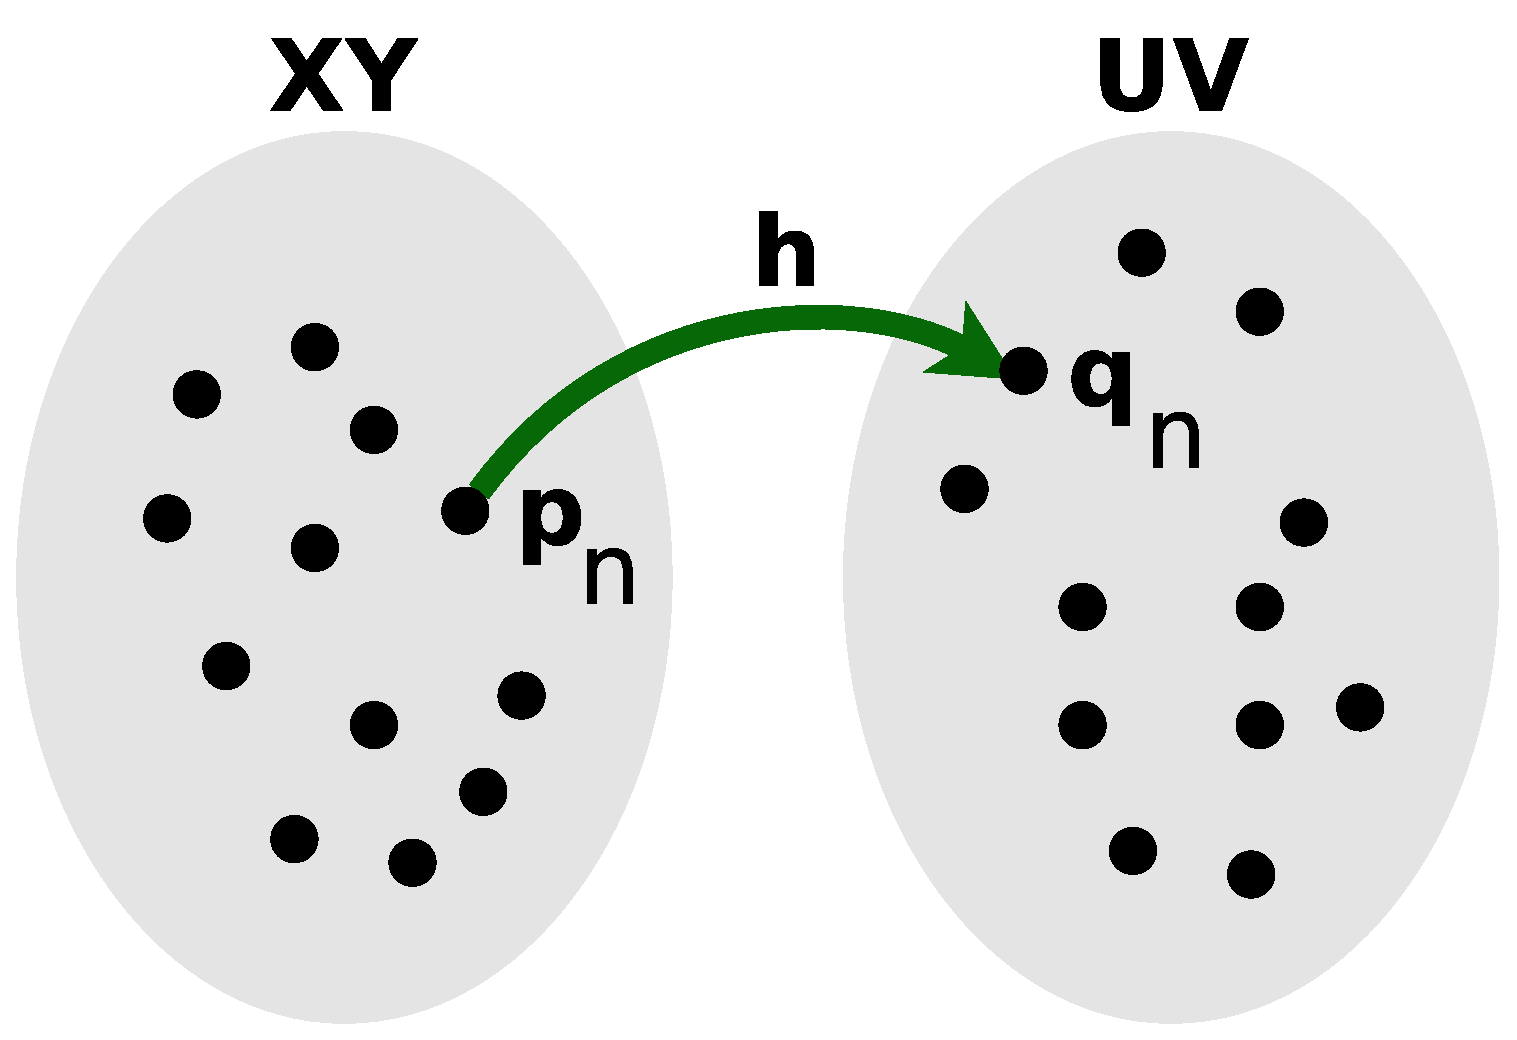
\includegraphics[width=0.8\linewidth]{chapters/inverso-mapeamento/mapeamento.eps} 
\end{minipage}
\begin{minipage}{0.6\textwidth}
\quad Se temos, $N$ pontos (amostras) $\VECTOR{p}_n=[x_n~~y_n]^{\transpose}\equiv (x_n,y_n)$ no plano $XY \in \mathbb{R}^2$, e
seus correspondentes $\VECTOR{q}_n=[u_n~~v_n]^{\transpose}\equiv (u_n,y_n)$
no plano $UV \in \mathbb{R}^2$ ,
$\forall n\in \{1, 2, 3, ..., N\}$, 
vinculados mediante a função $\VECTOR{f}(x,y): \mathbb{R}^2 \rightarrow \mathbb{R}^2$, 
que é um vetor função de transformação de coordenadas,
$\VECTOR{q}=\VECTOR{f}(\VECTOR{p})$, 
para um ponto $\VECTOR{p} \in XY$ qualquer e seu correspondente $\VECTOR{q} \in UV$.\\
\end{minipage}

Então, podemos modelar  
$[u~~v]^{\transpose} = \VECTOR{f}(\VECTOR{p})\equiv \VECTOR{f}(x,y)\equiv [f_1(x,y)~~f_2(x,y) ]^{\transpose}$, 
onde as funções $f_1(x,y)$ e $f_2(x,y)$ $: \mathbb{R}^2 \rightarrow \mathbb{R}$,
são polinômios\footnote{Os polinômios $f_1(x,y)$ e $f_2(x,y)$ são semelhantes, só a notação na escrita foi diferente.} de grau $M$,
\begin{equation}\label{eq:mapeamento:2}
\begin{matrix}
f_1(x,y) & = & +c_{1}\\
              ~ & ~ & +c_{2}~x + c_{3}~y\\
              ~ & ~ & +c_{4}~x^2 +c_{5}~xy + c_{6}~y^2\\
              ~ & ~ &  ...\\
              ~ & ~ & +\sum \limits_{l=0}^{M}c_{\left\{ \frac{M(M+1)}{2}+l+1\right\}}~x^{M-l}y^{l};
\end{matrix} 
\qquad
\begin{matrix}
f_2(x,y) & = & \sum \limits_{m=0}^{M} \sum \limits_{l=0}^{m}d_{\left\{ \frac{m(m+1)}{2}+l+1\right\}}~x^{m-l}y^{l}.
       ~ & ~ & ~\\
       ~ & ~ & ~\\
       ~ & ~ & ~\\
       ~ & ~ & ~\\
       ~ & ~ & ~
\end{matrix}
\end{equation}

Assim, o problema de conhecer $\VECTOR{f}(x,y)$ é equivalente ao 
problema de achar os vetores 
$\VECTOR{c}=[c_1~c_2~c_3~...~c_{\left\{ \frac{(M+1)(M+2)}{2}\right\}} ]^{\transpose}$ e
$\VECTOR{d}=[d_1~d_2~d_3~...~d_{\left\{ \frac{(M+1)(M+2)}{2}\right\}} ]^{\transpose}$;
com este fim são usadas as $N$ amostras $\VECTOR{p}_n$ e $\VECTOR{q}_n$,
para  procurar quais são os valores de $\VECTOR{c}$ e $\VECTOR{d}$
que provocam o mínimo erro nos escalares, 
$e_1(\VECTOR{c})$  e $e_2(\VECTOR{d})$.% $:\mathbb{R}^{\left\{ \frac{(M+2)(M+1)}{2}\right\}} \rightarrow \mathbb{R}$.
\begin{equation}\label{eq:mapeamento:3}
 e_1(\VECTOR{c})=||\MATRIX{A}\VECTOR{c}-\VECTOR{u}||^2 \qquad\qquad\qquad  e_2(\VECTOR{d})=||\MATRIX{A}\VECTOR{d}-\VECTOR{v}||^2,
\end{equation}
onde 
\begin{equation}\label{eq:mapeamento:4}
\VECTOR{u}=
\begin{bmatrix}
u_1 \\
u_2 \\
u_3 \\
\vdots \\
u_{N}
\end{bmatrix},
\qquad
\VECTOR{v}=
\begin{bmatrix}
v_1 \\
v_2 \\
v_3 \\
\vdots \\
v_{N}
\end{bmatrix},
\qquad
\MATRIX{A}=
\begin{bmatrix}
\VECTOR{a}_{10}     & \VECTOR{a}_{11}     & \dots  & \VECTOR{a}_{1M} \\
\VECTOR{a}_{20}     & \VECTOR{a}_{21}     & \dots  & \VECTOR{a}_{2M} \\
\VECTOR{a}_{30}     & \VECTOR{a}_{31}     & \dots  & \VECTOR{a}_{3M} \\
\vdots              & \vdots              & \ddots & \vdots \\
\VECTOR{a}_{N0} & \VECTOR{a}_{N1} & \dots  & \VECTOR{a}_{NM}
\end{bmatrix},
\end{equation}
\begin{equation}\label{eq:mapeamento:5}
\VECTOR{a}_{nm}=
\begin{bmatrix}
x^m_n  & x^{m-1}_n y_n  & x^{m-2}_n y^2_n    & \dots  & x^{1}_n y^{m-1}_n &  y^m_n 
\end{bmatrix}.
\end{equation}
Um caso especial é quando $\VECTOR{a}_{n0}=1$.
Assim, utilizando o Teorema \ref{theo:minAxbCAxb},
podemos achar o valor $\VECTOR{\hat{c}}$ e $\VECTOR{\hat{d}}$,
que minimizam as funções  $e_1(\VECTOR{\hat{c}})$  e $e_2(\VECTOR{\hat{d}})$:
\begin{equation}\label{eq:mapeamento:6}
\VECTOR{\hat{c}}=
\left[ \MATRIX{A}^{\transpose}  \MATRIX{A} \right]^{-1}\MATRIX{A}^{\transpose} \VECTOR{u},
\qquad \qquad \qquad \qquad
\VECTOR{\hat{d}}=
\left[ \MATRIX{A}^{\transpose}  \MATRIX{A} \right]^{-1}\MATRIX{A}^{\transpose} \VECTOR{v}.
\end{equation}

Devemos ter cuidado, pois para que exista uma solução única para $\VECTOR{\hat{c}}$ e $\VECTOR{\hat{d}}$,
o número de linhas de $\MATRIX{A}$ deve ser maior ou igual ao número de suas colunas\footnote{ Que
é equivalente ao número de elementos de $\VECTOR{\hat{c}}$ e $\VECTOR{\hat{d}}$}.
Assim, devemos escolher um valor $M$ que cumpra a seguinte relação com $N$,
\begin{equation}\label{eq:mapeamento:7}
N\geq \frac{(M+1)(M+2)}{2}.
\end{equation}
\end{theorem}

\begin{example}[ Mapeamento do polinomio 
$\VECTOR{f}(x,y)$ de grau $M=3$, para $N=15$ amostras:] ~\\
\begin{minipage}{0.38\textwidth}
\centering
\begin{tabular}{ |r |r || r |r|}
\hline
   $\VECTOR{x}$ & $\VECTOR{y}$ & $\VECTOR{u}$ & $\VECTOR{v}$ \\ \hline \hline
  -0.81 &-0.69 &-0.44 & 1.09 \\ 
   0.75 & 0.02 & 0.20 &-0.76 \\ 
   0.47 & 0.67 & 0.73 &-0.46 \\ 
   0.66 &-0.25 &-0.07 &-0.66 \\ 
  -0.76 & 0.73 &-0.91 &-0.63 \\ 
   0.10 &-0.72 &-0.50 & 0.20 \\ 
  -0.43 &-0.85 &-0.55 & 0.84 \\ 
   0.91 &-0.92 &-0.78 &-0.16 \\ 
   0.64 &-0.76 &-0.61 &-0.12 \\ 
  -0.79 &-0.28 &-0.35 & 0.46 \\ 
   1.00 &-0.27 & 0.08 &-0.75 \\ 
   0.84 &-0.11 & 0.13 &-0.75 \\ 
   0.79 & 0.95 & 1.79 & 0.79 \\ 
   0.65 &-0.90 &-0.82 & 0.06 \\ 
   0.76 &-0.95 &-0.88 & 0.03 \\ \hline
\end{tabular}
\end{minipage}
\begin{minipage}{0.61\textwidth}
Dadas $N=15$ amostras que representam pontos no plano $XY$ e seus correspondentes 
no plano $UV$, como pode ser visto na tabela da esquerda;
se desejamos obter um polinômio $\VECTOR{f}(x,y)$ de grau $M=3$,
que mapeie ambos conjuntos de pontos; podemos usar a Eq. (\ref{eq:mapeamento:6}) 
para resolver este problema.
Porem, antes de iniciar o procedimento, devemos usar a Eq. (\ref{eq:mapeamento:7}),
para corroborar que $15 \geq (3+1)(3+2)/2\equiv 10$.

Assim usando a Eq. (\ref{eq:mapeamento:6}) obtemos o vetor $\VECTOR{\hat{c}}=$ 
\begin{center}
\begin{tabular}{ r r r r }
  \hline
  -0.060306 &   0.240624 &   0.260580 &  -0.117630 \\ \hline
   0.996594 &  -0.089543 &   0.304348 &  -0.128405 \\ \hline
   0.464804 &   0.481949 & ~ & ~ \\ \hline
\end{tabular}
\end{center}

e o vetor $\VECTOR{\hat{d}}=$ 
\begin{center}
\begin{tabular}{ r r r r }
\hline
  -0.70762 &  -0.37822 &  -0.96840 &   0.57036 \\ \hline
   0.90987 &   0.83260 &  -0.21166 &   0.49152  \\ \hline
   0.55825 &   0.39762 & ~ & ~ \\ \hline
\end{tabular}
\end{center}
Que provocam um erro de mapeamento para $\VECTOR{u}$ e $\VECTOR{v}$,
de $0.73\%$ e $0.61\%$, respetivamente.
\end{minipage}
\end{example}


